\documentclass[11pt,a4paper]{article}
\usepackage[a4paper, total={6in, 8in}]{geometry}
\usepackage{amssymb}
\usepackage{makeidx}
\usepackage{amsfonts}
\usepackage{amsmath}
\usepackage{amsthm}
\usepackage{graphicx}
\usepackage[dvips]{epsfig}
\usepackage{longtable}
\usepackage{graphics}
\usepackage{multirow}
\usepackage[section]{placeins}
\usepackage{graphicx}				
\usepackage{amssymb}
\usepackage{mathtools}
\usepackage{tensor}
\usepackage{float}


% for comments
\usepackage{todonotes} 
\newcommand{\taariq}[1]{\todo[inline,color=green!20!white]{\textbf{Taariq:} #1}}
\newcommand{\nils}[1]{\todo[inline,color=blue!20!white]{\textbf{Nils:} #1}}

%Title
\def\university#1{{\sl \begin{center} #1 \vspace{5pt} \end{center} } }
\def\inst#1{\vspace{1pt} \unskip$^{#1}$}

\newtheorem{theorem}{Theorem}
\newtheorem{lemma}{Lemma}
\newtheorem{proposition}{Proposition}
\newtheorem{corollary}{Corollary}
\newtheorem{definition}{Definition}
\newtheorem{assumption}{Assumption}
\newtheorem{example}{Example}
\newtheorem{remark}{Remark}

%Commands
\renewcommand{\P}{\operatorname{P}}
\newcommand{\calF}{\mathcal{F}}
\newcommand{\calG}{\mathcal{G}}
\newcommand{\calH}{\mathcal{H}}
\newcommand{\calT}{\mathcal{T}}
\newcommand{\calD}{\mathcal{D}}
\newcommand{\calA}{\mathcal{A}}
\newcommand{\calL}{\mathcal{L}}
\newcommand{\calR}{\mathcal{R}}
\newcommand{\calP}{\mathcal{P}}


% Modes of convergence
\newcommand{\distr}{\stackrel{d}{\to}}
\newcommand{\as}{\stackrel{\textrm{a.s.}}{\to}}
\newcommand{\inprob}{\stackrel{\P}{\to}}
\newcommand{\weakly}{\stackrel{w}{\to}}
\newcommand{\diag}{\operatorname{diag}}
\newcommand{\Tr}{\operatorname{Tr}}

% Distributions
\newcommand{\NegMult}{\operatorname{NegMult}}
\newcommand{\NegBin}{\operatorname{NegBin}}
\newcommand{\Pois}{\operatorname{Pois}}
\newcommand{\Mult}{\operatorname{Mult}}
\newcommand{\Normal}{\operatorname{N}}

%%% SYMBOLS
\newcommand{\R}{\mathbb{R}}  % The real numbers.
\newcommand{\E }{\mathbb{E}}  % Expectation Operator
\renewcommand{\P}{\mathbb{P}}  % Probability
\newcommand{\Cov}{\operatorname{Cov}}  % Cov Operator
\newcommand{\Var}{\operatorname{Var}}  % Var Operator
\newcommand{\MSEPin}{\textbf{MSEP}_{\text{in}}}
\newcommand{\MSEPOin}{{\textbf{MSEP}^0}_{\text{in}}}
\newcommand{\MSEPIin}{\textbf{MSEP}^1_{\text{in}}}
\newcommand{\MSEP}{\textbf{MSEP}}
\newcommand{\MSE}{\textbf{MSE}}
\newcommand{\eqdis}{\stackrel{d}{=}}

\newcommand{\bigzero}{\mbox{\normalfont\Large\bfseries 0}}
\newcommand{\bigone}{\mbox{\normalfont\Large\bfseries I}}

\title{A stopping rule for regression trees}
\author{Mathias Lindholm, Taariq Nazar, Filip Lindskog, Nils Engler}


%\date{}


\begin{document}
\maketitle

\begin{abstract}

\end{abstract}

% keywords
\noindent {\bf Keywords}: overfitting, covariance-penalties, cost-complexity parameters

\section{Introduction}

\section{An iterative stopping test statistic}\label{sec:test_stat}

Consider a random covariate-response pair $(X, Y)$ taking values in $\R^{d} \times \R$. Assume fixed covariate trainings data $x_1, \dots, x_N$ and iid trainings-response-data $Y_1, \dots, Y_N $ satisfying 
$$
\calL(Y_i) = \calL\left(Y \mid X = x_i \right)  = \Normal(\mu(x_i), \sigma^2)
$$
for an unknown regression function $\mu \colon \R^d \to \R$ and unknown $\sigma^2 > 0$. Let $(X^*, Y^*)$ be iid with respect to $(X, Y)$ and independent of $(Y_i)_{i=1}^N$.

Suppose we have a disjoint partition $ \bigcup_{j=1}^J D_j = \R^d$ and a tree regressor
\begin{align}\label{eq:mu_hat_0}
\hat \mu_0(x) = \hat \mu_0(x, (x_i, Y_i)_{i=1}^N) = \sum_{j=1}^J I\{x \in D_j\} \hat m_j,
\end{align}
where $\hat m_j = \frac{1}{n_{D_j}} \sum_{i = 1}^{N} Y_i I\{x_i \in D_j\}$ with $n_{D_j} = |\{i \colon x_i \in D_j  \}|$. 
%Here, we have assumed without loss of generality that $x_1, \dots, x_{n_{D_j}} \in D_1, x_{n_1 + 1}, \dots, x_{n_{D_j}} \in D_2$ etc. 
Let
\begin{align*}
\mu_{D_j} = \E[Y \mid X \in D_j ], \quad \sigma^2_{D_j} = \E[(Y-\mu_{D_j})^2 \mid X \in D_j]
= \Var(Y \mid X \in D_j).
 \end{align*}
 Note that $\hat \mu(x)$ is a random variable since it is a function of the trainings-responses $(Y_i)_{i=1}^N$. Denote by 
 $$
 \MSEP^0_j = \E \left[
\left(Y^* - \hat \mu_0(X^*)\right)^2 \mid X^* \in D_j
 \right] 
 $$ 
 the generalization error of the predictor $\hat \mu_0$, given region $D_j$.
\begin{lemma}\label{lem:mot1}
Then,
\begin{align*}
\MSEP^0_j =  \sigma_{D_j}^2\left(1 + \frac{1}{n_{D_j}}\right). 
\end{align*}
\end{lemma}

Fix a region $j$ and let $A_j \dot \cup B_j = D_j$ be a split at the terminal node $j$. Let $\hat \mu_1$ be defined as in \eqref{eq:mu_hat_0}, but with $J+1$ regions after splitting node $j$. As above, define the generalization error of $\hat \mu_1$, given $D_j$,
 $$
 \MSEP^1_j = \E \left[
\left(Y^* - \hat \mu_1(X^*)\right)^2 \mid X^* \in D_j
 \right].
 $$ 

\begin{lemma}\label{lem:MSEP1}
Then,
\begin{align*}
\MSEP^1_j = \sigma_{A_j}^2\left(1 + \frac{1}{n_{A_j}}\right)\pi_{A_j \mid D_j} + \sigma_{B_j}^2\left(1 + \frac{1}{n_{B_j}}\right)\pi_{B_j \mid D_j},
\end{align*}
where $\pi_{A_j\mid D_j} = \P(X \in A_j \mid X \in D_j)$ and analogous for $\pi_{B_j \mid D_j}$.
\end{lemma}

The split at node $j$ increased the mean squared error of prediction (generalisation error) in region $D_j$, if 
\begin{align}\label{eq:stop_criterion}
\MSEP^0_j < \MSEP^1_j.
\end{align}
Estimating the unknown parameters $\sigma_{A_j}^2, \pi_{A_j \mid D_j}$ by the unbiased estimators 
\begin{align}\label{eq:par_estimators}
\hat \sigma_{A_j}^2 = \frac{1}{n_{A_j} - 1} \sum_{i \colon x_i \in A_j} (Y_i - \overline Y_{A_j})^2, \quad  \hat \pi_{A_j \mid D_j} = n_{A_j}/n_{D_j},
\end{align}
where $\overline Y_{A_j} = 1/n_A \sum_{i \colon x_i \in A_j} Y_i$, and similarly for $\sigma_{B_j}^2, \pi_{B_j \mid D_j}$,
this motivates the stopping test statistic
\begin{align}\label{eq:R_j}
R_j = \frac{\widehat \MSEP^1_j}{\widehat \MSEP^0_j} = \frac{(n_{A_j} +1) \hat \sigma^2_{A_j} + (n_{B_j} +1) \hat \sigma^2_{B_j}}{(n_{D_j} +1) \hat \sigma^2_{D_j}}
\end{align}
for a split at node $j$. Following \eqref{eq:stop_criterion}, the interpretation of $R_j \gg 1$ is that, with a high probability, the generalization error has increased after splitting.

\subsection{An alternative motivation: Covariance penalties}
Let $Y_1^*, \dots, Y_N^*$ be independent, independent of $(Y_i)_{i=1}^N$ and satisfying $\calL(Y_i^*) = \calL(Y_i)$ for $i=1, \dots, N$. Here, $(Y_i)_{i=1}^N$ is defined as in the beginning of section \ref{sec:test_stat}. Define the in-sample mean squared error of prediction before and after a split at node $j$ by 
\begin{align*}
{\MSEPOin}_{,j} = \frac{1}{n_{D_j}} \sum_{i \colon x_i \in D_j} (Y_i^* - \hat \mu_0(x_i))^2, \quad
{\MSEPIin}_{,j} = \frac{1}{n_{D_j}} \sum_{i \colon x_i \in D_j} (Y_i^* - \hat \mu_1(x_i))^2.
\end{align*}

%Hence, writing $\mu_i = \mu(x_i)$ for $i=1, \dots, N$, $(Y_i)_{i=1}^N$ follows a multivariate normal distribution with
%$$
%	\mu = (\mu_1, \dots, \mu_N)^T, \quad \Sigma = \sigma^2 I_N.
%$$

\begin{lemma}\label{lem:mot2}
Then,
\begin{align*}
\E[{\MSEPOin}_{,j}]
 = &\sigma_{D_j}^2\left(1 + \frac{1}{n_{D_j}}\right), \\
\E[{\MSEPIin}_{,j}] =  &\sigma_{A_j}^2\left(1 + \frac{1}{n_{A_j}}\right)\pi_{A_j \mid D_j} + \sigma_{B_j}^2\left(1 + \frac{1}{n_{B_j}}\right)\pi_{B_j \mid D_j},
\end{align*}
where $\pi_{A_j\mid D_j} = \P(X \in A_j \mid X \in D_j)$ and analogous for $\pi_{B_j \mid D_j}$.
\end{lemma}
Choosing the same estimators as in \eqref{eq:par_estimators}, this approach hence motivates the same stopping testing statistic $R_j$ as in \eqref{eq:R_j}.




\subsection{Signal/No-signal hypothesis testing}


\subsection{The distribution function under the Null-Hypothesis}
For the sake of readibility, we keep node $j$ fixed and drop it from the notation in the following. That is, we denote $n_{D_j}$ by $n$, and $n_{A_j}, n_{B_j}$ by $n_A$, $n_B$. Let
$$
F^0_R(r) = \P_0(R \leq r)
$$
be the distribution function of the stopping test statistic $R$ from \eqref{eq:R_j}, given $H_0$ holds true.
\begin{lemma}
It holds that
\begin{align*}
F_R^0(r) = \P_0(Z_r \leq 0), 
\end{align*}
where, under $H_0$,
\begin{align}\label{eq:Z_r}
	Z_r \eqdis
	\lambda_A^r \chi^2_{n_A -1}
	+ \lambda_B^r \tilde \chi^2_{n_B -1}
	+ \lambda_{\text{neg}}^r \bar \chi_1^2,
\end{align}
with
\begin{align*}
	\lambda_A^r =             \frac{n_A +1}{n_A -1} - r\frac{n+1}{n-1}, \quad 
		\lambda_B^r =             \frac{n_B +1}{n_B -1} - r\frac{n+1}{n-1}, \quad
	\lambda_{\text{neg}}^r = & -r\frac{n+1}{n-1}
\end{align*}
and $\chi^2_{n_A -1}$, $\tilde \chi^2_{n_B -1}$ and $\bar \chi_1^2$ are independent chi-squared distributed random variables.
\end{lemma}

The next result shows large sample size properties of $R$.
\begin{lemma}[Large sample size]\label{lem:large_sample}
Let $n \to \infty$ and assume that $n_{A} /n \to a \in (0, 1)$, $n_B/n \to 1 - a$. Then, under $H_0$, $R$ converges to $1$ in probability.
\end{lemma}
This is in line with the numerical results in Figure \ref{fig:F_R}.

\begin{figure}[H]
\centering
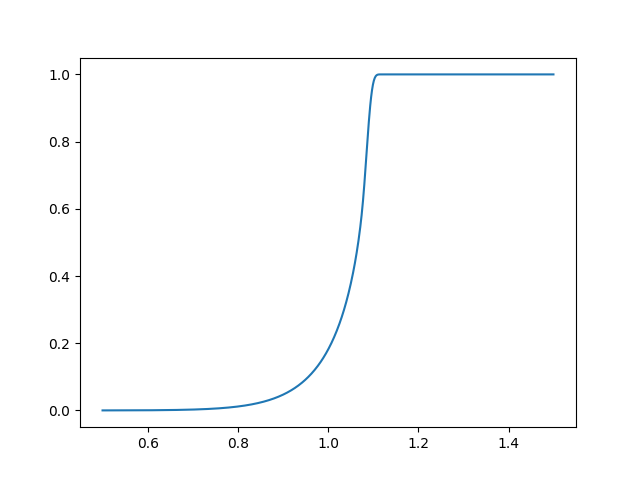
\includegraphics[width=.5\textwidth]{./Figures/10_13_F_R.png}\hfill
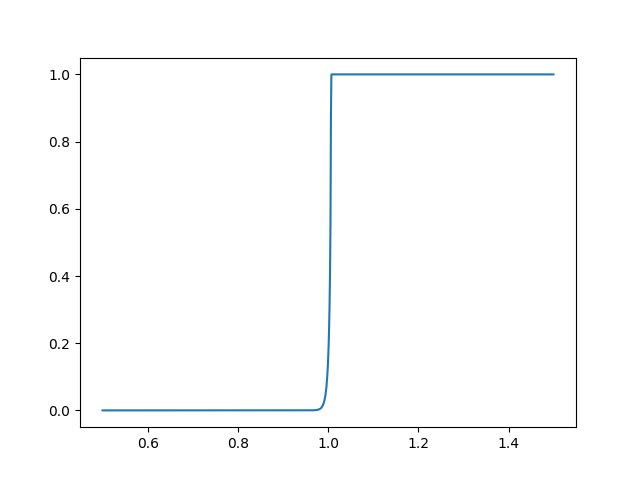
\includegraphics[width=.5\textwidth]{./Figures/160_170_F_R.png}\hfill
\caption{$F_R^0(r)$ for $(n_A, n_B) = (10, 13)$ and $(n_A, n_B) = (160, 170)$.}
\label{fig:F_R}
\end{figure}

Figure \ref{fig:F_R_2} shows how the distributions change when $n_A, n_B$ vary while $n$ is fixed. It seems that low quantiles are not much affected by unbalancedness of $(n_A, n_B)$.

\begin{figure}[H]
\centering
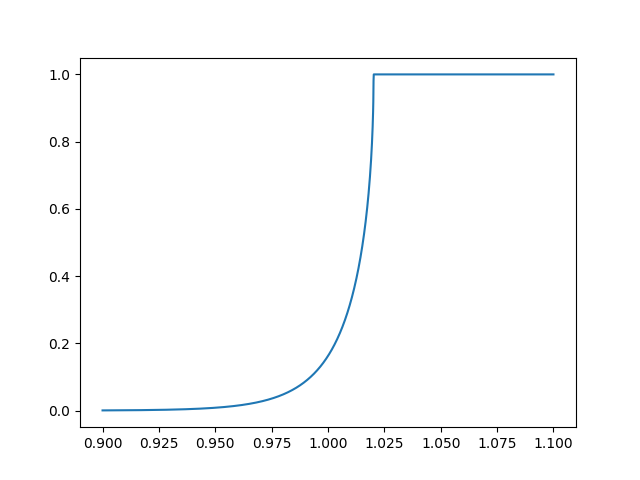
\includegraphics[width=.5\textwidth]{./Figures/50_50_F_R.png}\hfill
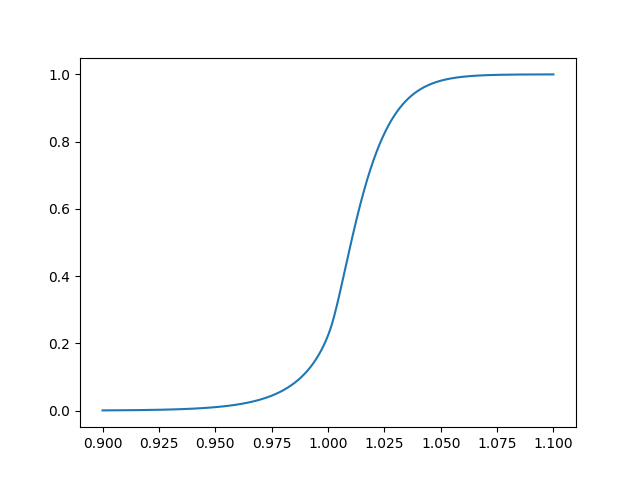
\includegraphics[width=.5\textwidth]{./Figures/95_5_F_R.png}\hfill
\caption{$F_R^0(r)$ for $(n_A, n_B) = (50, 50)$ and $(n_A, n_B) = (95, 5)$.}
\label{fig:F_R_2}
\end{figure}



\section{The stopping rule}

\section{Numerical illustration}

\section{Appendix: Proofs}

\begin{proof}[Proof of Lemma \ref{lem:large_sample}]
Let $n \to \infty$ and assume that $n_A /n \to a \in (0, 1)$, $n_B/n \to 1 - a$. We first want to investigate the weak limit of $Z_{r}$ under $H_0$, i.e. the limit of 
\begin{align}\label{eq:Z_lim}
\tilde \lambda_A^r \frac{\chi_{n_A - 1}}{n_A - 1} + \tilde \lambda_B^r \frac{\tilde \chi_{n_B - 1}}{n_B - 1} + \lambda_{\text{neg}}^r \bar \chi_{1},
\end{align}
where all chi-squares are independent and 
\begin{align*}
\tilde \lambda_A^r = &\frac{(n_A + 1)(n-1) - r(n+1)(n_A-1)}{n-1}, \\
\tilde \lambda_B^r = &\frac{(n_B + 1)(n-1) - r(n+1)(n_B-1)}{n-1}, \quad \lambda_{\text{neg}}^r = -r \frac{n+1}{n-1}.
\end{align*}
The first two standardised chi-squares in \eqref{eq:Z_lim} each converge to $1$ in probability. Moreover,
\begin{align*}
&\lambda_{\text{neg}}^r \to - r, \\
&\tilde \lambda_A^r = \frac{2 n_B}{n-1} + \frac{(1-r)(n+1)(n_A - 1)}{n-1}
\to 
\begin{cases}
2(1-a), & r=1 \\
- \infty, & r >1 \\
+ \infty, & r <1
\end{cases}
\end{align*}
and similarly
\begin{align*}
\tilde \lambda_B^r 
\to 
\begin{cases}
2a, & r=1 \\
- \infty, & r >1 \\
+ \infty, & r <1.
\end{cases}
\end{align*}
Hence, under $H_0$, we get convergence in distribution by the Slutzky Theorem
\begin{align*}
Z_{r} \to Z_{r}^\infty := 
\begin{cases}
2 - \bar \chi_{1}, & r=1 \\
- \infty, & r >1 \\
+ \infty, & r <1.
\end{cases}
\end{align*}
Since $Z_{r}^\infty$ has no mass at $0$ for any $r > 0$, this implies that 
\begin{align*}
F_R^0(r) = \P_0(Z_{r} \leq 0) \to \P_0(Z_{r}^{\infty} \leq 0) = 
\begin{cases}
\P(\bar \chi_{1} \geq 2), & r=1 \\
1, & r >1 \\
0, & r <1.
\end{cases}
\end{align*}
This shows that the ratio $R$ converges to $1$ under $H_0$ in distribution (and hence in probability). Note that the limit does not depend on $a$.

\end{proof}



\begin{thebibliography}{99}

\end{thebibliography}

\end{document}



